%% Template para dissertacao/tese na classe UFBAthesis
%% versao 1.0
%% (c) 2005 Paulo G. S. Fonseca
%% (c) 2012 Antonio Terceiro
%% (c) 2014 Christina von Flach
%% www.dcc.ufba.br/~flach/ufbathesis

%% Carrega a classe ufbathesis
%% Opcoes: * Idiomas
%%           pt   - portugues (padrao)
%%           en   - ingles
%%         * Tipo do Texto
%%           bsc  - para monografias de graduacao
%%           msc  - para dissertacoes de mestrado (padrao)
%%           qual - exame de qualificacao de mestrado
%%           prop - exame de qualificacao de doutorado
%%           phd  - para teses de doutorado
%%         * Media
%%           scr  - para versao eletronica (PDF) / consulte o guia do usuario
%%         * Estilo
%%           classic - estilo original a la TAOCP (deprecated) - apesar de deprecated, manter esse.
%%           std     - novo estilo a la CUP (padrao)
%%         * Paginacao
%%           oneside - para impressao em face unica
%%           twoside - para impressao em frente e verso (padrao)

% Atenção: Manter 'classic' na declaracao abaixo:
\documentclass[bsc, en, classic, a4paper]{ufbathesis}

%% Preambulo:
\usepackage[utf8]{inputenc}
\usepackage{graphicx}
\usepackage{hyphenat}
\usepackage{booktabs}
\usepackage{pifont}
\usepackage{multirow}
\usepackage{listings} 
\usepackage{colortbl}
\usepackage{xfrac}
\usepackage[printonlyused, withpage]{acronym}

% Custom preamble
\usepackage{tikz}
\usetikzlibrary{positioning}
\tikzset{block/.style={draw,thick,text width=2cm,minimum height=1cm,align=center},
line/.style={-latex}
}

% Universidade
\university{Universidade Federal da Bahia}

% Endereco (cidade)
\address{Salvador}

% Instituto ou Centro Academico
\institute{Instituto de Matem\'{a}tica e Estatística}

% Nome da biblioteca - usado na ficha catalografica
\library{Biblioteca Reitor Mac\^{e}do Costa} %TODO: is this correct?

% Programa de pos-graduacao %TODO: is this correct?
\program{Programa de Graduação em Ciência da Computação}

% Area de titulacao
\majorfield{Ci\^{e}ncia da Computa\c{c}\~{a}o}

% Titulo da dissertacao
\title{Pluggable Thread Scheduling Agents for the Java Virtual Machine}

% Data da defesa
% e.g. \date{19 de fevereiro de 2013}
\date{TODO} % TODO
% e.g. \defenseyear{2013}
\defenseyear{TODO} % TODO

% Autor
% e.g. \author{Jose da Silva}
\author{Denilson das Merc\^{e}s Amorim}

% Orientador(a)
% Opcao: [f] - para orientador do sexo feminino
% e.g. \adviser[f]{Profa. Dra. Maria Santos}
\adviser{Vinicius Tavares Petrucci}

% Orientador(a)
% Opcao: [f] - para orientador do sexo feminino
% e.g. \coadviser{Prof. Dr. Pedro Pedreira}
% Comente se nao ha co-orientador
%\coadviser{Nome Completo do CO-ORIENTADOR}

%% Inicio do documento
\begin{document}

\pgcompfrontpage

%% Parte pre-textual
\frontmatter

\presentationpage

%%%%%%%%%%%%%%%%%%%%%%%%%
% Ficha catalografica
%%%%%%%%%%%%%%%%%%%%%%%%%

\authorcitationname{Amorim, Denilson das Merc\^{e}s} % e.g. Terceiro, Antonio Soares de Azevedo
\advisercitationname{Petrucci, Vinicius Tavares} % e.g. Chavez, Christina von Flach Garcia
%\coadvisercitationname{Sobrenome, Nome do CO-ORIENTADOR} % e.g. Mendonca, Manoel Gomes de
\catalogtype{Monografia (Graduação)} % e.g. ``Tese (Doutorado)''

\catalogtopics{TODO} % Listar palavras-chave do trabalho para a FICHA CATALOGRAFICA}, por exemplo, ``1. Complexidade Estrutural. 2. Qualidade de Software 3. Engenharia de Software''
\catalogcdd{XXX.XX} % e.g.  XXX.XX (número nesse formato serah dado pela biblioteca)
\catalogcdu{XXX.XX.XXX} % e.g.  XXX.XX.XXX (idem) 
\catalogingsheet

%%%%%%%%%%%%%%%%%%%%%
% Termo de aprovacaoo
%%%%%%%%%%%%%%%%%%%%%

%TODO
%\approvalsheet{Salvador, 14 de dezembro de 2018}{
%   \comittemember{Prof. Dr. Maurício Pamplona Segundo}{Universidade Federal da Bahia}
%   \comittemember{Prof. Dr. Professor 2}{Universidade Federal da Bahia}
%   \comittemember{Profa. Dra. Professora 3}{Universidade Federal da Bahia}
   % Para mestrado, apenas 3.
   % \comittemember{Prof. Dr. Professor 4}{Universidade HJKL}
   % \comittemember{Profa. Dra. Professora 5}{Universidade QWERTY}
%}

%%%%%%%%%%%%%%%%%%%%%%%%%%%%%%%%%%%%%%%%
% Dedicatoria, Agradecimentos, Epigrafe
%%%%%%%%%%%%%%%%%%%%%%%%%%%%%%%%%%%%%%%%

% Agradecimentos
% Se preferir, crie um arquivo `a parte e o inclua via \include{}
\acknowledgements
%TODO: write acknowledgements
TODO

%%%%%%%%%%%%%%%%%%%%%
% Resumo em Portugues
%%%%%%%%%%%%%%%%%%%%%

\resumo
TODO


% TODO
\begin{keywords}
TODO
\end{keywords}

%%%%%%%%%%%%%%%%%%%
% Resumo em Ingles
%%%%%%%%%%%%%%%%%%%

\abstract
TODO

\begin{keywords}
TODO
\end{keywords}

%%%%%%%%%%%%%%%%%%%
% Sumario / Indice
%%%%%%%%%%%%%%%%%%%

% Comente para ocultar
\tableofcontents

% Lista de figuras
% Comente para ocultar
\listoffigures

% Lista de tabelas
% Comente para ocultar
\listoftables


\iffalse
\chapter*{Lista de Siglas}

% Sintaxe da lista de acordo com a documentação do pacote `acronym'
% documentação: http://mirror.unl.edu/ctan/macros/latex/contrib/acronym/acronym.pdf
\begin{acronym}[PGCOMP]
    \acro{PGCOMP}{Programa de Pós-Graduação em Ciência da Computação}
    \acro{CNPq}{Conselho Nacional de Desenvolvimento Centífico e Tecnológico}
\end{acronym}
\fi

%% Parte textual
\mainmatter

%\input{content-sample}
\xchapter{Introduction}{}

% According to data from Alibaba’s datacenter, more than 90% of latency-critical cloud services are written and deployed as Java applications [17 - Who Limits the Resource Efficiency of My Datacenter: An Analysis of Alibaba Datacenter Traces]

% Describe chapters

\section{Motivation}

The idea of sharing the time resources of a computer machine is one of the oldest in computer science. Huge and expensive computers were underused both by the limited speed of human interaction \cite{strachey1959time} and by programs accessing slow peripherals devices \cite{codd1960multiprogram}. Both problems led to the development of computer systems capable of executing multiple tasks in a single processing unit concurrently through time slicing \cite{corbato1962experimental,codd1959multiprogramming}.

Today, small computer chips are not only capable of running multiple tasks in a single processing unit, but multiple tasks in multiple processing units thanks to chip multithreading \cite{tullsen1995simultaneous,olukotun1996case}. This paradigm required, and still requires, further research in task scheduling algorithms to take proper advantage of chips \cite{fedorova2004chip}. On top of that, the subject has recently gained more attention due to the rising interest in reducing power consumption of data-centers and embedded systems \cite{mittal2014power,mittal2014survey}. Modern chip designers are heavily invested in adjusting their cores for this purpose \cite{greenhalgh2011big,fisher2005power} with architectural features such as asymmetric multi-core processing \cite{kumar2003single}, dynamic voltage scaling \cite{macken1990voltage} and per-core power gating \cite{leverich2009power}.

Given the interest for research in scheduling algorithms and the barriers during the implementation of one, such as the need to modify the operating system kernel or develop runtime systems to control applications, this work presents an infrastructure on top of the Java Virtual Machine made specifically to fasten the development of scheduling algorithms. This way, researches can focus on the algorithms instead of the supporting environment.


\section{Related Work}

%% Scheduling
% Compiler-assisted Adaptive Program Scheduling in big.LITTLE Systems
% Hipster: Hybrid Task Manager for Latency-Critical CloudWorkloads


%% TODO profilers and java profilers

%% Profilers with user-customized code
% + An Efficient and Generic Event-based Profiler Frameworkfor Dynamic Languages
% + Portable and accurate samplingprofiling for Java
% + A Portable CPU-ManagementFramework for Java
% + ProfBuilder:  A Package for Rapidly Building Java ExecutionProfilers

%% Path tracing and CCT
% + Exploiting  Hardware  Performance  Counters  with  Flow  and  Context  Sensitive  Profiling 
% A Portable Sampling-Based  Profiler for Java Virtual Machines

%% Async
% https://dl.acm.org/doi/pdf/10.1145/2568088.2576759

% Related:
% Sampling Profiler API for sw/hw counters (remember openmp stuff?)

\section{Contribution}

% Applications go here

TODO

\xchapter{Background}{}


\section{Process Scheduling}

%single process in the system. In the face of the first problem, time-shared systems were developed to support concurrent users in a single machine \cite{corbato1962experimental}. For the latter, the concept of multi-programming was developed.



%\subsection{Processor core scheduling}

%\subsubsection{Single core processors}

%\subsubsection{Symmetric multi-core processors}

%\subsubsection{Asymmetric multi-core processors}

\section{Java Virtual Machine}

% https://homepages.cwi.nl/~boncz/msc/2020-ChristianStuart.pdf Section 2.1.3

% SAFE POINTS
% https://psy-lob-saw.blogspot.com/2014/03/where-is-my-safepoint.html
% http://psy-lob-saw.blogspot.com/2015/12/safepoints.html
% http://psy-lob-saw.blogspot.com/2016/02/why-most-sampling-java-profilers-are.html
% http://psy-lob-saw.blogspot.com/2016/06/the-pros-and-cons-of-agct.html
% http://blog.ragozin.info/2012/10/safepoints-in-hotspot-jvm.html

% https://bugs.openjdk.java.net/browse/JDK-8178287

% https://assets.ctfassets.net/oxjq45e8ilak/4mfbX5FJuw0A8M00UK4uKa/ce60f2cab12408e01ce927e90ebb2f7a/Andrey_Pangin__Vadim_Tsesko._The_Art_of_JVM_Profiling.pdf

% Profiling is used in JITs (may be usefl to write about this?)

\subsection{VM Phases}

% TODO

\subsection{Java Threads}

% http://openjdk.java.net/groups/hotspot/docs/RuntimeOverview.html#Thread%20Management|outline
% https://www.oracle.com/technetwork/java/whitepaper-135217.html

% Paper: Evaluating the Accuracy of Java Profilers

\subsection{Synchronization Primitives}

% Efficient Tracing and Versatile Analysis of Lock Contention in Java Applications on the Virtual Machine Level -- https://dl.acm.org/doi/pdf/10.1145/2851553.2851559


\subsubsection{Monitors}

\subsubsection{Thread Parking}

\subsection{Java Native Interface}

% Explain COM-like nature (interface pointer)

\subsection{JVM Tool Interface}

% Explain the docs in few words
% and more

% Cite from docs that it doesn't include full-speed method entry/exit (maybe in introduction/methodology?)

% Phase

% Callback safe

\section{Elasticsearch}

\section{Instrumentation}

% INSTRUMENTATION MAY BE USED NOT ONLY FOR PROFILING BUT FOR OTHER THINGS (WHAT?)
% CODE COVERAGE


\section{Profiling}

% https://homepages.cwi.nl/~boncz/msc/2020-ChristianStuart.pdf Section 2.2

% EXPLAIN THAT PROFILERS CAN BE STATISTICAL, INSTRUMENTATION, ETC
% PROFILERS CAN BE OF STORAGE, MEMORY, HEAP, NETWORK, ENERGY, CPU, ETC

% OTHER USES: SCHEDULER, GARBAGE COLLECTOR, JIT COMPILERS


\section{Synchronization}

%\subsection{Non-blocking synchronization}

TODO



% EXPLAIN WHY NOT USING JVMTI EXTENSION MECHANISM

\xchapter{Methodology}{}

In this chapter, we present the design (Section~\ref{sec:design}) and implementation (Section~\ref{sec:impl}) of JVMTIPROF.

\section{Design} \label{sec:design}

JVMTIPROF follows a similar design to the JVMTI. Agents create environments, and those environments have capabilities, events, and other functionalities. Once the environment is disposed, all the associated capabilities are relinquished and events disabled.

\subsection{Startup \& Shutdown}

JVMTIPROF must be used from within a JVMTI agent. During \jvmtihref{startup}{agent startup}, when a JVMTI environment is created, a JVMTIPROF environment can be injected into the JVMTI one. This is achieved through the \apihref{Create}{\code{jvmtiProf_Create}} function. This function modifies the JVMTI environment, and returns an accompanying function table that can be used to access JVMTIPROF functionality. JVMTI functionality can continue to be accessed through its own function table.

During \jvmtihref{shutdown}{agent shutdown}, the JVMTIPROF environment must be disposed through the \apiref{DisposeEnvironment} function. Unlike JVMTI, the disposal must be done explicitly since the JVM doesn't know about the existence of JVMTIPROF. However, if the JVMTI environment is disposed explicitly (through its own \apijvmtiref{DisposeEnvironment}), the associated JVMTIPROF environment is automatically disposed. Disposal of the JVMTIPROF environment can be done at any time, not only during agent shutdown.

\subsection{Functionality}

JVMTIPROF provides events that can be used to intercept individual methods and sample the execution of the application.

It also provides functions that can be used to get accurate call stack trace of a thread, which can be used during sampling.

Similarly to the JVMTI, events can be set through the \apiref{SetEventNotificationMode} and \apiref{SetEventCallbacks} functions. Capabilities necessary for the event to work properly must be added through the \apiref{AddCapabilities} function.

Details on the programming interface can be found in the appendix (Appendix~\ref{chap:api}). An example agent that samples execution and prints call stack traces can be found in listing~\ref{lst:example_execution_sampling}.

\subsubsection*{Execution Sampling}

To sample the application, the agent must enable and set callbacks for the event \apieventref{SampleExecution}, as well as add the \code{can_generate_sample_execution_events} capability. An agent may, optionally, set the sampling interval through the \apiref{SetExecutionSampingInterval} function.


To obtain call stack traces, an agent must possess the necessary capability and invoke \apiref{GetStackTraceAsync}. This function differs from JVMTI's \apijvmtiref{GetStackTrace} in that it can be used during sampling. This avoids the safepoint bias present in most Java profilers.


\lstinputlisting[language=C++,frame=tb,caption=Example agent that uses JVMTIPROF to sample the application and print its call trace. Error handling is omitted for brevity.,label=lst:example_execution_sampling]{src/listing/demo-sample-execution.cpp}.

\subsubsection*{Method Interception}

JVMTI provides functionality to intercept \emph{all} Java methods (i.e. \apijvmtiref{MethodEntry}), but it significantly degrades performance. JVMTIPROF introduces a low overhead alternative capable of intercepting individual methods.

To intercept a Java method, an agent must obtain the method identifier and use \apiref{SetMethodEventFlag} to enable entry and/or exit events on such method. The method identifier can be obtained through JNI's \jnihref{getmethodid}{\code{GetMethodID}}. Alongside the flag, the associated event notification, callback and capabilities must be set.

\section{Implementation} \label{sec:impl}

\subsection{JVMTI Injection}

JVMTIPROF uses events and capabilities from JVMTI to implement some of its functionaliites. Therefore the JVMTI environment must be modified for JVMTIPROF and JVMTI functionalities to co-exist. For example, method interception is achieved through JVMTI's \apijvmtiref{ClassFileLoadHook} event. As such, an end-programmer wouldn't be able to use the same event for its own purpose, but since we modify JVMTI, an end-programmer can also use events that are in use by JVMTIPROF.

This is achieved by modifying function pointers in the JVMTI function table to point to functions managed by JVMTIPROF. The \apijvmtiref{DisposeEnvironment}, \apijvmtiref{SetEventCallbacks}, \apijvmtiref{SetEventNotificationMode}, \apijvmtiref{RetransformClasses}, \apijvmtiref{RedefineClasses}, \apijvmtiref{GetCapabilities}, \apijvmtiref{AddCapabilities} and \apijvmtiref{RelinquishCapabilities} functions are modified. This injection process occurs during the \apihref{Create}{\code{jvmtiProf_Create}} function.

\subsubsection*{Environment Disposal}

JVMTI's \apijvmtiref{DisposeEnvironment} is modified such that it also disposes the associated JVMTIPROF environment.

\subsubsection*{Event Management}

The \apijvmtiref{SetEventCallbacks} function is modified such that event callbacks in use by JVMTIPROF don't end up replaced . Instead, the pointer to these newly set callbacks are stored, and whenever JVMTIPROF's callback for that event is called, the stored callback is also invoked. This way, both JVMTIPROF and the end-programmer can be notified about a JVMTI event.

The \apijvmtiref{SetEventNotificationMode} hook works in a similar manner. It avoids replacing notification modes in use by JVMTIPROF, and instead stores them internally. When an event used by both occurs, the modes set by the end-programmer are inspected to decide whether the callback stored by \apijvmtiref{SetEventCallbacks} should be called.

\subsubsection*{Capabilitiy Management}

The capabilities functions are modified to avoid exposing capabilities set by JVMTIPROF to the end-programmer. The JVMTI's \apijvmtiref{GetCapabilities} should return an empty set of capabilities even though JVMTIPROF has set some of them (e.g. \jvmtihref{jvmtiCapabilities.can_retransform_classes}{\code{can_retransform_classes}}). \apijvmtiref{RelinquishCapabilities} must not relinquish capabilities possessed by JVMTIPROF. The state of relinquished capabilities is mainted internally by JVMTIPROF such that \apijvmtiref{GetCapabilities} can return a view that is according to what the end-programmer expects. \apijvmtiref{AddCapabilities} is also modified for this purpose.

% TODO what happens above is kinda of a trampoline. Use that word.

\subsubsection*{Class Redefinition}

The \apijvmtiref{RetransformClasses} and \apijvmtiref{RedefineClasses} may need to be hooked in order to force allocation of method identifiers after class redefinition (or retransformation). This is explained in detail at Section~\ref{sec:impl_callstacktrace}.

\subsection{Method Interception}

JVMTIPROF provides the ability to notify the end-programmer about method calls of interest. This is achieved by instrumenting the bytecode of the method such that its epilogue and prologue includes calls to a JVMTIPROF managed function. When the JVMTIPROF function is called, the method call event is sent upstream to the end-programmer.

The target methods are set through JVMTIPROF's \apiref{SetMethodEventFlag}, and when the bytecode of the class associated with the method is being loaded, it is instrumented to include JVMTIPROF's internal calls. Class loading is intercepted through JVMTI's  \apijvmtiref{ClassFileLoadHook} event. If the class is already loaded, the event is forced by calling JVMTI's \apijvmtiref{RetransformClasses} on the class to be instrumented.

\medskip
\begin{lstlisting}[language=Java,frame=tb,escapechar=@,captionpos=b,caption=Example instrumentation applied by method interception. Instrumented code is in green. The \code{sum} method is modified such that JVMTIPROF is notified about entries and exits on it.,label=lst:method_interception_instrumentation]
@\color{patchadd}public class JVMTIPROF \{@
    @\color{patchadd}static native void onMethodEntry(long methodID);@
    @\color{patchadd}static native void onMethodExit(long methodID);@
@\color{patchadd}\}@

public class Example {

    @\color{patchadd}final long sumMethodID = /* determined at runtime */;@

    public int sum(int a, int b) {
        @\color{patchadd}JVMTIPROF.onMethodEntry(sumMethodID);@
        @\color{patchadd}try \{@
            return a + b;
        @\color{patchadd}\} finally \{@
            @\color{patchadd}JVMTIPROF.onMethodExit(sumMethodID);@
        @\color{patchadd}\}@
    }
}
\end{lstlisting}

An illustration of the instrumentation performed is given in Listing~\ref{lst:method_interception_instrumentation}. JVMTIPROF defines a new class with native methods to communicate back with C++. The method exit notification is enclosed in a \code{try...finally} block such that exceptions do not cause the event to be missed. The identifier of the hooked method is passed as argument to JVMTIPROF since that information is part of the event sent upstream, enabling the end-programmer to identify which method has been entered or exited.



% TODO future work: create one JVMTIPROF function dynamically for each hook


\subsection{Execution Sampling}

JVMTIPROF provides an event to simplify the setup of sampling profilers. It is implemented by the means of a high-precision CPU timer (\code{CLOCK_PROCESS_CPUTIME_ID}) and a notification signal (\code{SIGPROF}). The timer is set to expire every interval nanoseconds (as set by \apiref{SetExecutionSampingInterval}), and once expired, the application receveis a signal at the thread that caused the timer to expire.

The event handler is then invoked from the signal handler. Since the event is received in an async-signal, its code must be async-signal-safe. That is, it must not perform memory allocations, acquire locks, or perform any other operation that may interfere with the interrupted thread. This restricts the event handler to primitive operations and async-signal-safe system calls. The handler must be careful to not consume much CPU time as well, since it is blocking the execution of the thread, safepoint polling, and the receiving of other signals. As such, the handler set by the end-programmer must, in most cases, simply push the sampling information of interest (e.g. stack trace) into a queue, which can be consumed later (e.g. by a sampling thread) in a non-async-signal context.

% TODO future work: per-thread sampling

\subsection{Call Stack Trace} \label{sec:impl_callstacktrace}

JVMTI offers a function to obtain call stack traces of the Java application (\apijvmtiref{GetStackTrace}). However, it cannot be used during execution sampling since it performs non-async-signal-safe operations, such as memory allocations. To mitigate this, some profilers do not use async-signals and instead spawn a thread that takes call traces every few milliseconds.

This tends to produce meaningless profilers for many reasons. First, \apijvmtiref{GetStackTrace} blocks untils all of the threads to trace from are in a safepoint. The more threads to trace, the greater the artificial slowdown. Secondly, the traces taken are always at lines of code which are safepoints, implying innacurate results.

JVMTIPROF introduces \apiref{GetStackTraceAsync}, a function capable of taking stack traces in async-signal contexts. This means traces can be taken at non-safepoints, such as in the execution sampling event handler.

\subsubsection*{AsyncGetCallTrace}

Oracle's HotSpot JVM provides an unsupported internal API capable of async-signal-safe stack tracing. It is famously known as \code{AsyncGetCallTrace} (AGCT for short). JVMTIPROF makes use of such API to implement its \apiref{GetStackTraceAsync}. As a downside, this functionality isn't supported in other JVM implementations.

AGCT requires all method identifiers to be pre-allocated, since it cannot perform memory allocations in an async-singal context. JVMTI's \apijvmtiref{ClassLoad} and \apijvmtiref{ClassPrepare} events are used for this purposes. \apijvmtiref{RetransformClasses} and \apijvmtiref{RedefineClasses} are also hooked in the JVMTI function table to re-allocate identifiers after class redefinition.

\subsubsection*{Debugging Non-Safepoints}

For AGCT to work, the JVM command-line flag \code{-XX:+DebugNonSafepoints} must be present. This option instructs the JVM to produce debug information for lines of code which aren't regarded as safepoints. This debug information allows AGCT to map addresses of JIT compiled code to bytecode locations.

The setting of this flag in JVMTIPROF is achieved by enabling JVMTI's \apijvmtiref{CompiledMethodLoad} event. This event has the side-effect of enabling debugging information on non-safepoints. 

% TODO cite https://github.com/openjdk/jdk/blob/2f3e494b80cce8e357ceac9a897c42d7e8f54af5/src/hotspot/share/prims/forte.cpp#L519-L670
% TODO can improve https://github.com/jvm-profiling-tools/async-profiler/blob/55da899511d6e427d87c85f6ef6b08ea6a0c1746/src/profiler.cpp#L343
% TODO -XX:+UnlockDiagnosticVMOptions -XX:+DebugNonSafepoints still necessary if agent is attached.

% TODO future work: Windows support

\xchapter{Evaluation}{}
\label{cap:evaluation}

In this chapter, we evaluate JVMTIPROF by using it to instrument Elasticsearch. A profile-guided frequency scaling solution~\cite{hurryupccgrid} is adapted to use JVMTIPROF instead of JVMTI. We then measure the overhead and identify whether JVMTIPROF can produce the same gains as the baseline despite its abstractions.

\section{Experimental Setup}

We conduct experiments on a bare-metal server instance provided by the Chameleon Cloud service. The server consists of an Intel Xeon Gold 6126 (Skylake architecture) with 196GB of DRAM and a 220GB SSD disk. We run Ubuntu 20.04 (Linux kernel 5.4) and Elasticsearch version 6.5.4. For the search index database, we use the Wikipedia dump version \code{enwiki-latest-pages-articles} downloaded in September 2022.

The CPU has 24 physical cores equally divided between two sockets. Intel's Hyperthreading technology is turned off, so we only consider the physical core count. To isolate the network effects in the shared experimental platform, we configure socket 0 to run the server-side applications (Elasticsearch) and socket 1 to execute the load generator (FABAN).

Energy measurement is done through Intel's Running Average Power Limit (RAPL) interface. We measure the energy consumption counter at the beginning and end of the experiment, and the difference between those two values is considered the energy consumed for that particular experiment.

The client, FABAN~\cite{faban}, is responsible for generating query requests with randomized keywords, ranging from 1 to 18 keywords, under a Zipfian distribution.

The load generation process consisted of 20-minute runs of continuous search queries. The FABAN workload generator is used to create four clients, with each client issuing, on average, one request per second. The goal is to analyze the behavior of each solution, considering a single request at a time. An additional configuration of three times the requests-per-seconds is used to explore loads similar to that of production environments.

We perform six runs for each combination of load and solution and report the mean and standard deviation of the 99-percentile latency and energy consumption.

\section{Baseline}

We use the Linux Ondemand power governor and Hurryup~\cite{hurryupccgrid} as baselines for our experiments. Hurryup is a profile-guided frequency scaling solution for Elasticsearch that outperforms Ondemand on energy consumption while attaining acceptable levels of tail latency constraints.

Hurryup works by instrumenting Elasticsearch's hot functions to produce enter and exit events. A runtime scheme uses these events to adapt the individual processor core frequencies. In our experiments, we observe Hurryup saving up to 25\% in energy compared to Linux's Ondemand governor, as seen in Figure~\ref{fig:ondem_vs_hup}.

\begin{figure}[hb]
\centering
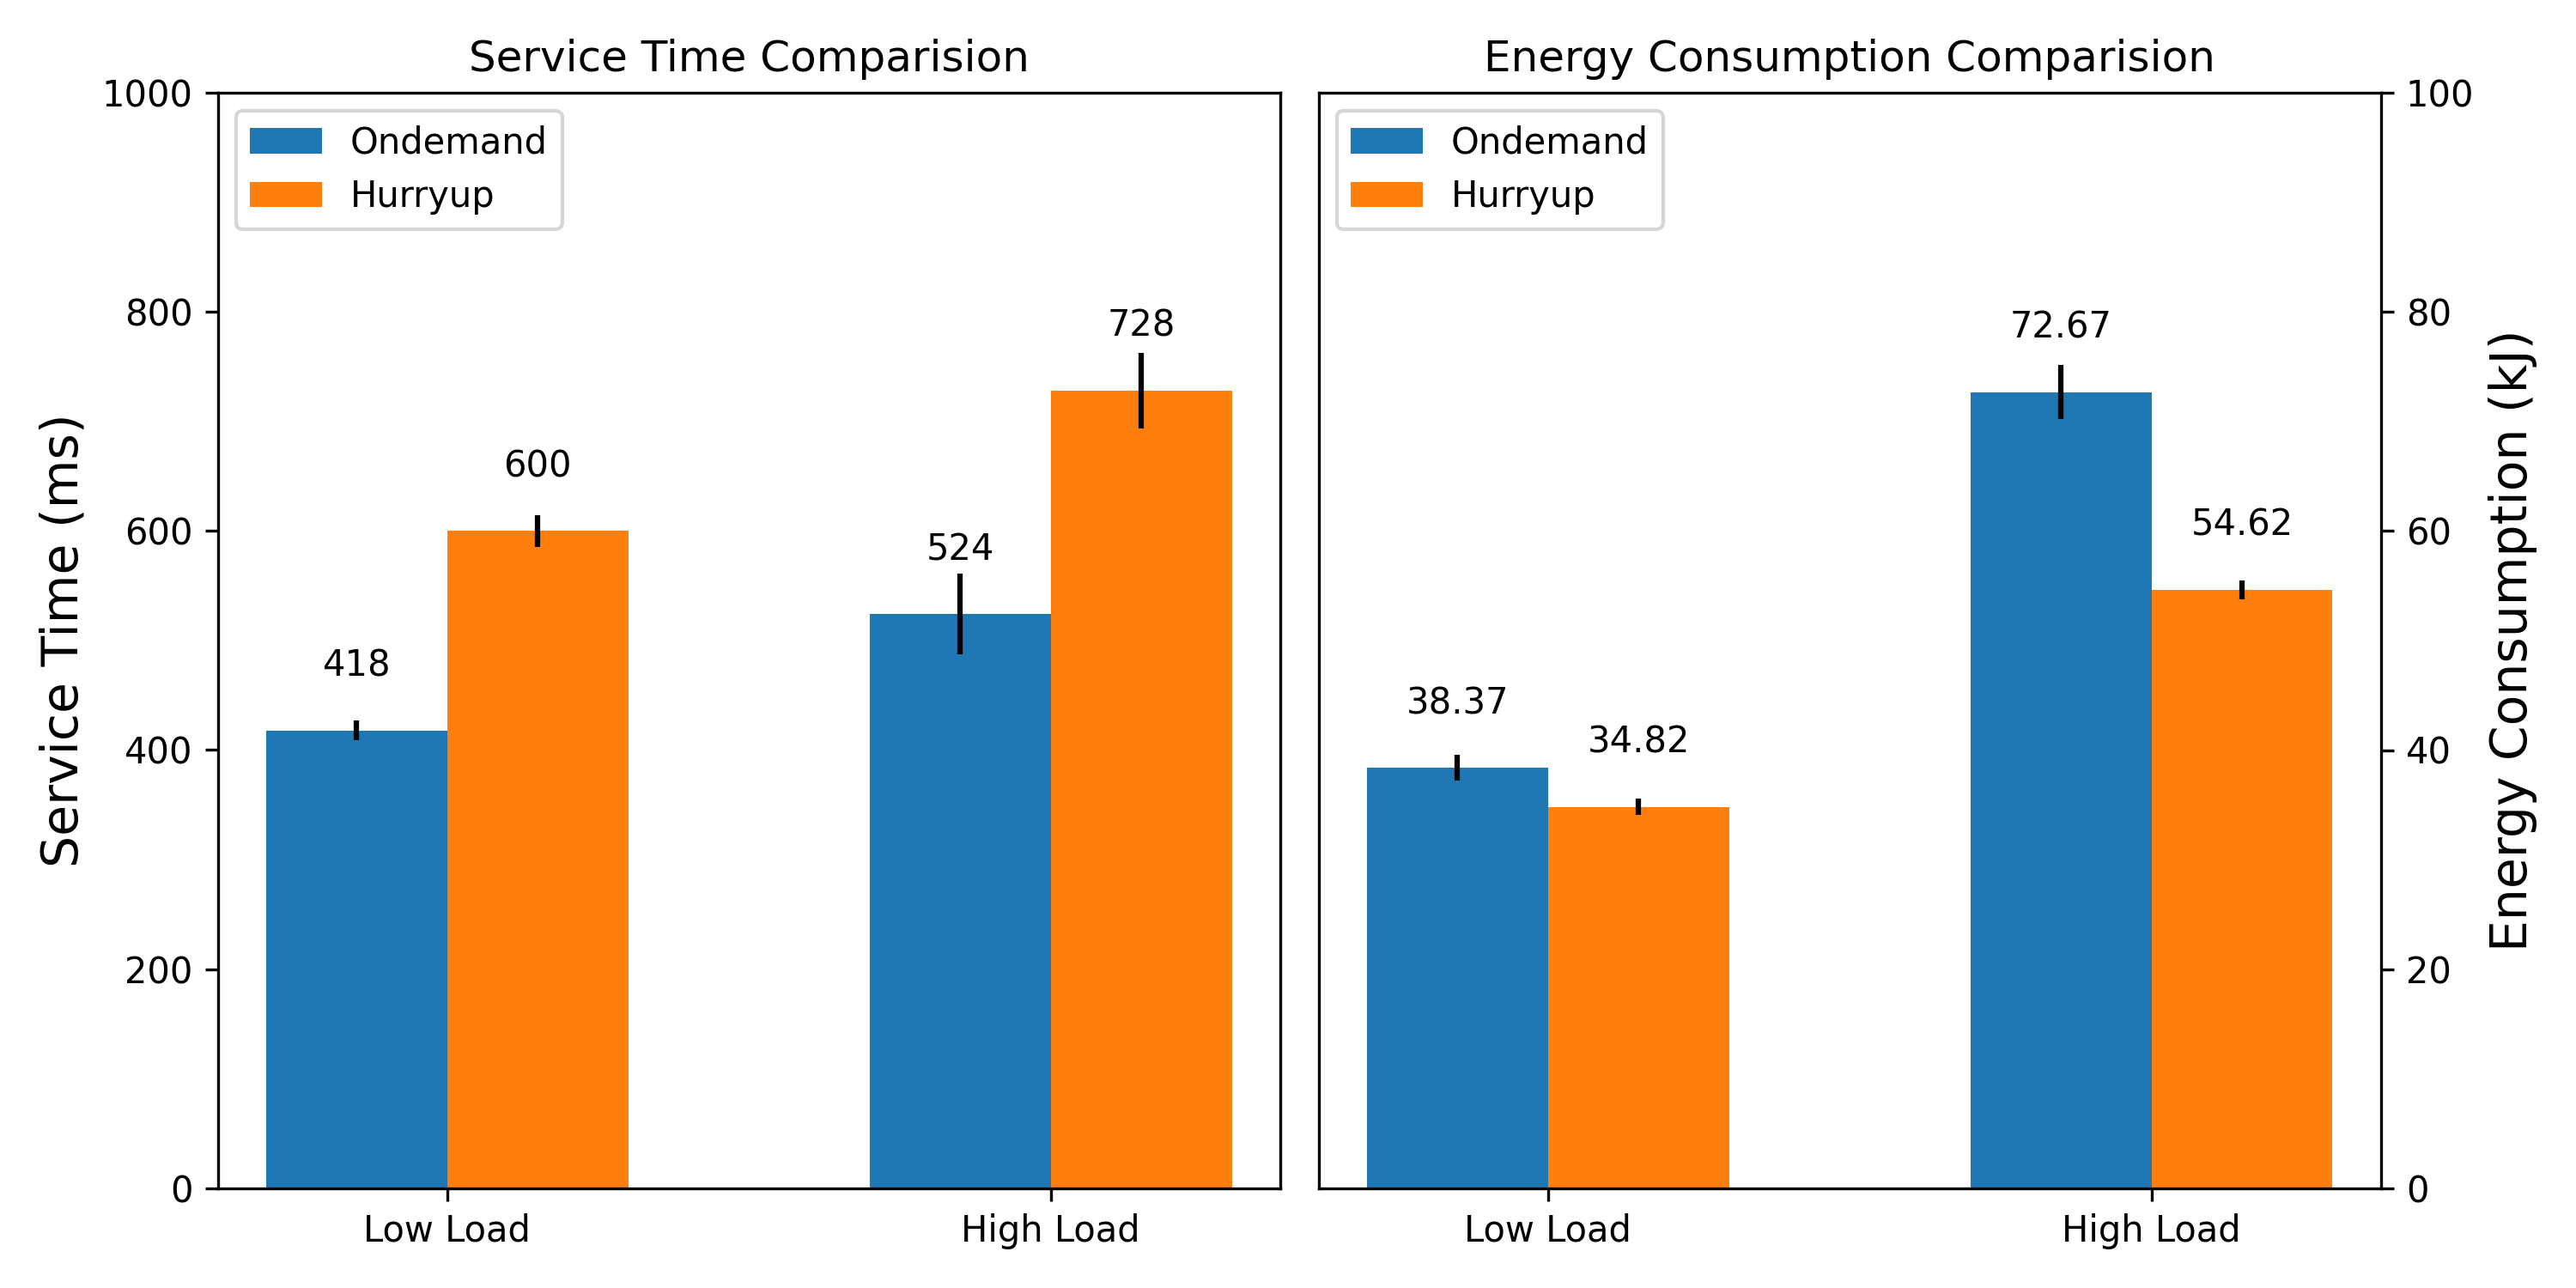
\includegraphics[width=1.0\textwidth]{src/figure/ondem_vs_hup.png}
\caption{An experiment comparing Linux's Ondemand governor against Hurryup's frequency scaling scheme. The left plot presents Elasticsearch's service time, and the right plot the energy consumption of the CPU while executing search requests. Results are shown for both a low and high server load.}
\label{fig:ondem_vs_hup}
\end{figure}

\section{Results}

We modify Hurryup to use JVMTIPROF's instrumentation methods and re-execute the experiments as reported in Figure~\ref{fig:ondem_vs_hup_vs_newhup}. We notice that JVMTIPROF can be similar to or slightly worse than JVMTI in the context of Hurryup but can still achieve energy gains compared to Ondemand.

\begin{figure}[ht]
\centering
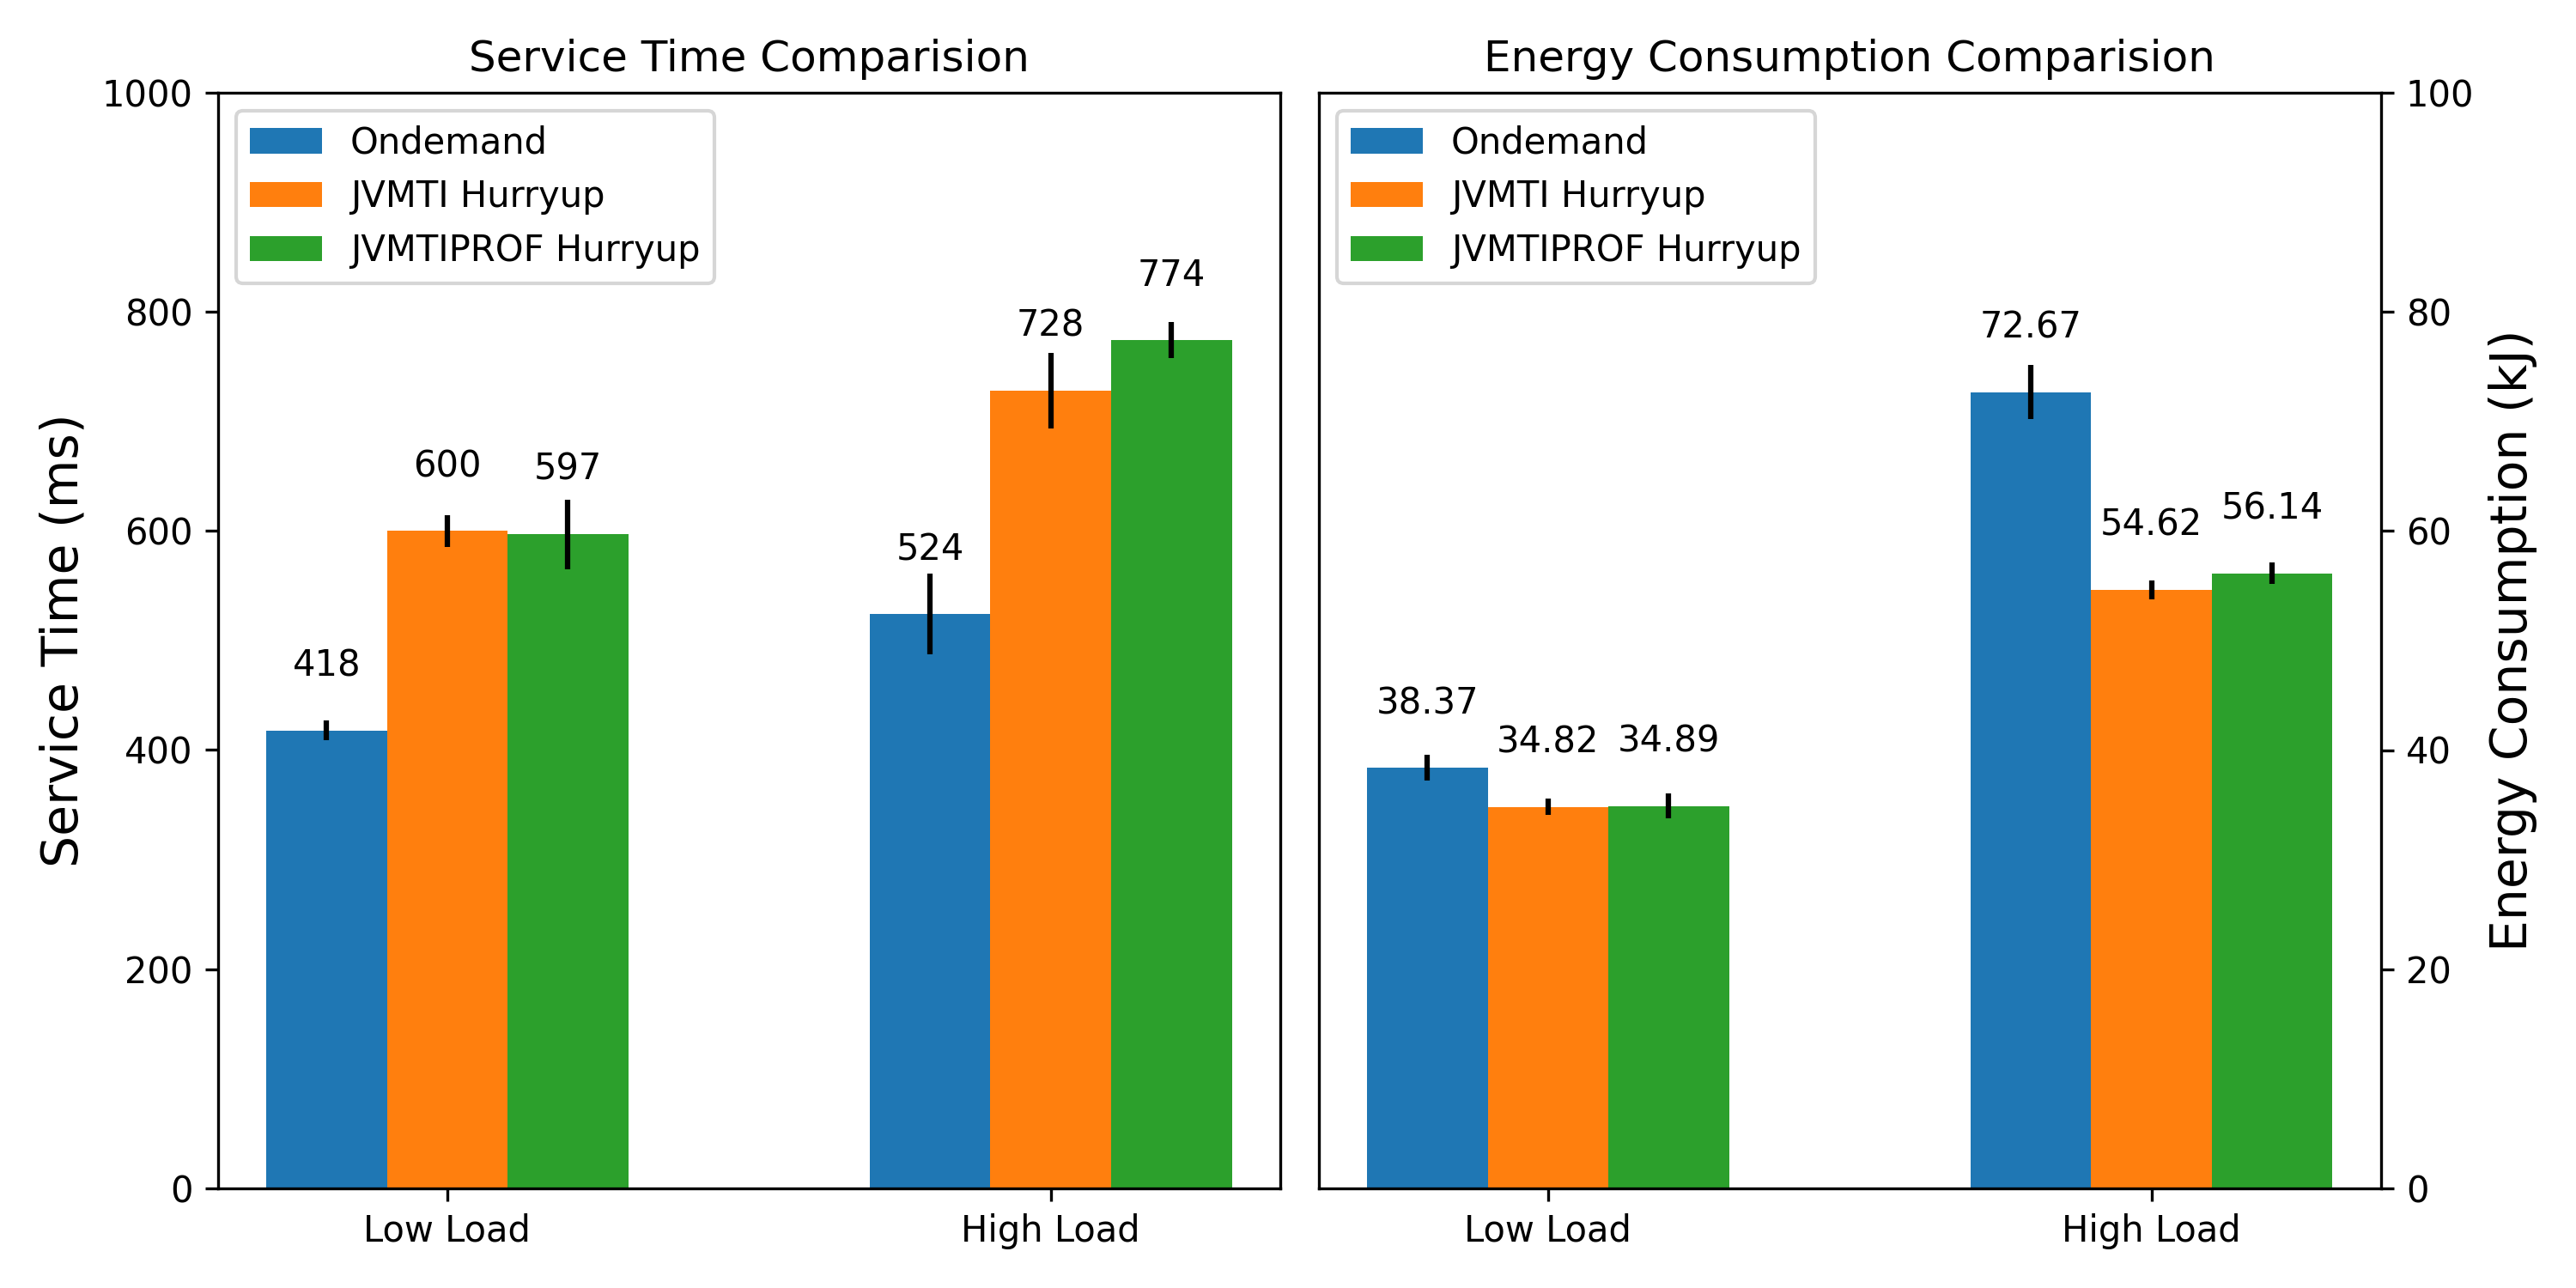
\includegraphics[width=1.0\textwidth]{src/figure/ondem_vs_hup_vs_newhup.png}
\caption{An experiment comparing Hurryup's performance when implemented with JVMTIPROF versus the baseline. The left plot presents Elasticsearch's service time, and the right plot the energy consumption of the CPU while executing search requests. Results are shown for both a low and high server load.}
\label{fig:ondem_vs_hup_vs_newhup}
\end{figure}

At a lower load, the JVMTI and JVMTIPROF implementations do not present a statistically significant difference in service time and energy consumption. When tripling the load, the JVMTIPROF version can be 6\% worse in service time and 2.78\% worse in energy consumption.

We also compare the overhead of instrumenting Elasticsearch's hot functions, excluding Hurryup-specific logic. Results are presented in Figure~\ref{fig:overhead}. There is no statistically significant difference between instrumenting or not instrumenting said functions with either JVMTI or JVMTIPROF.

\begin{figure}[ht]
\centering
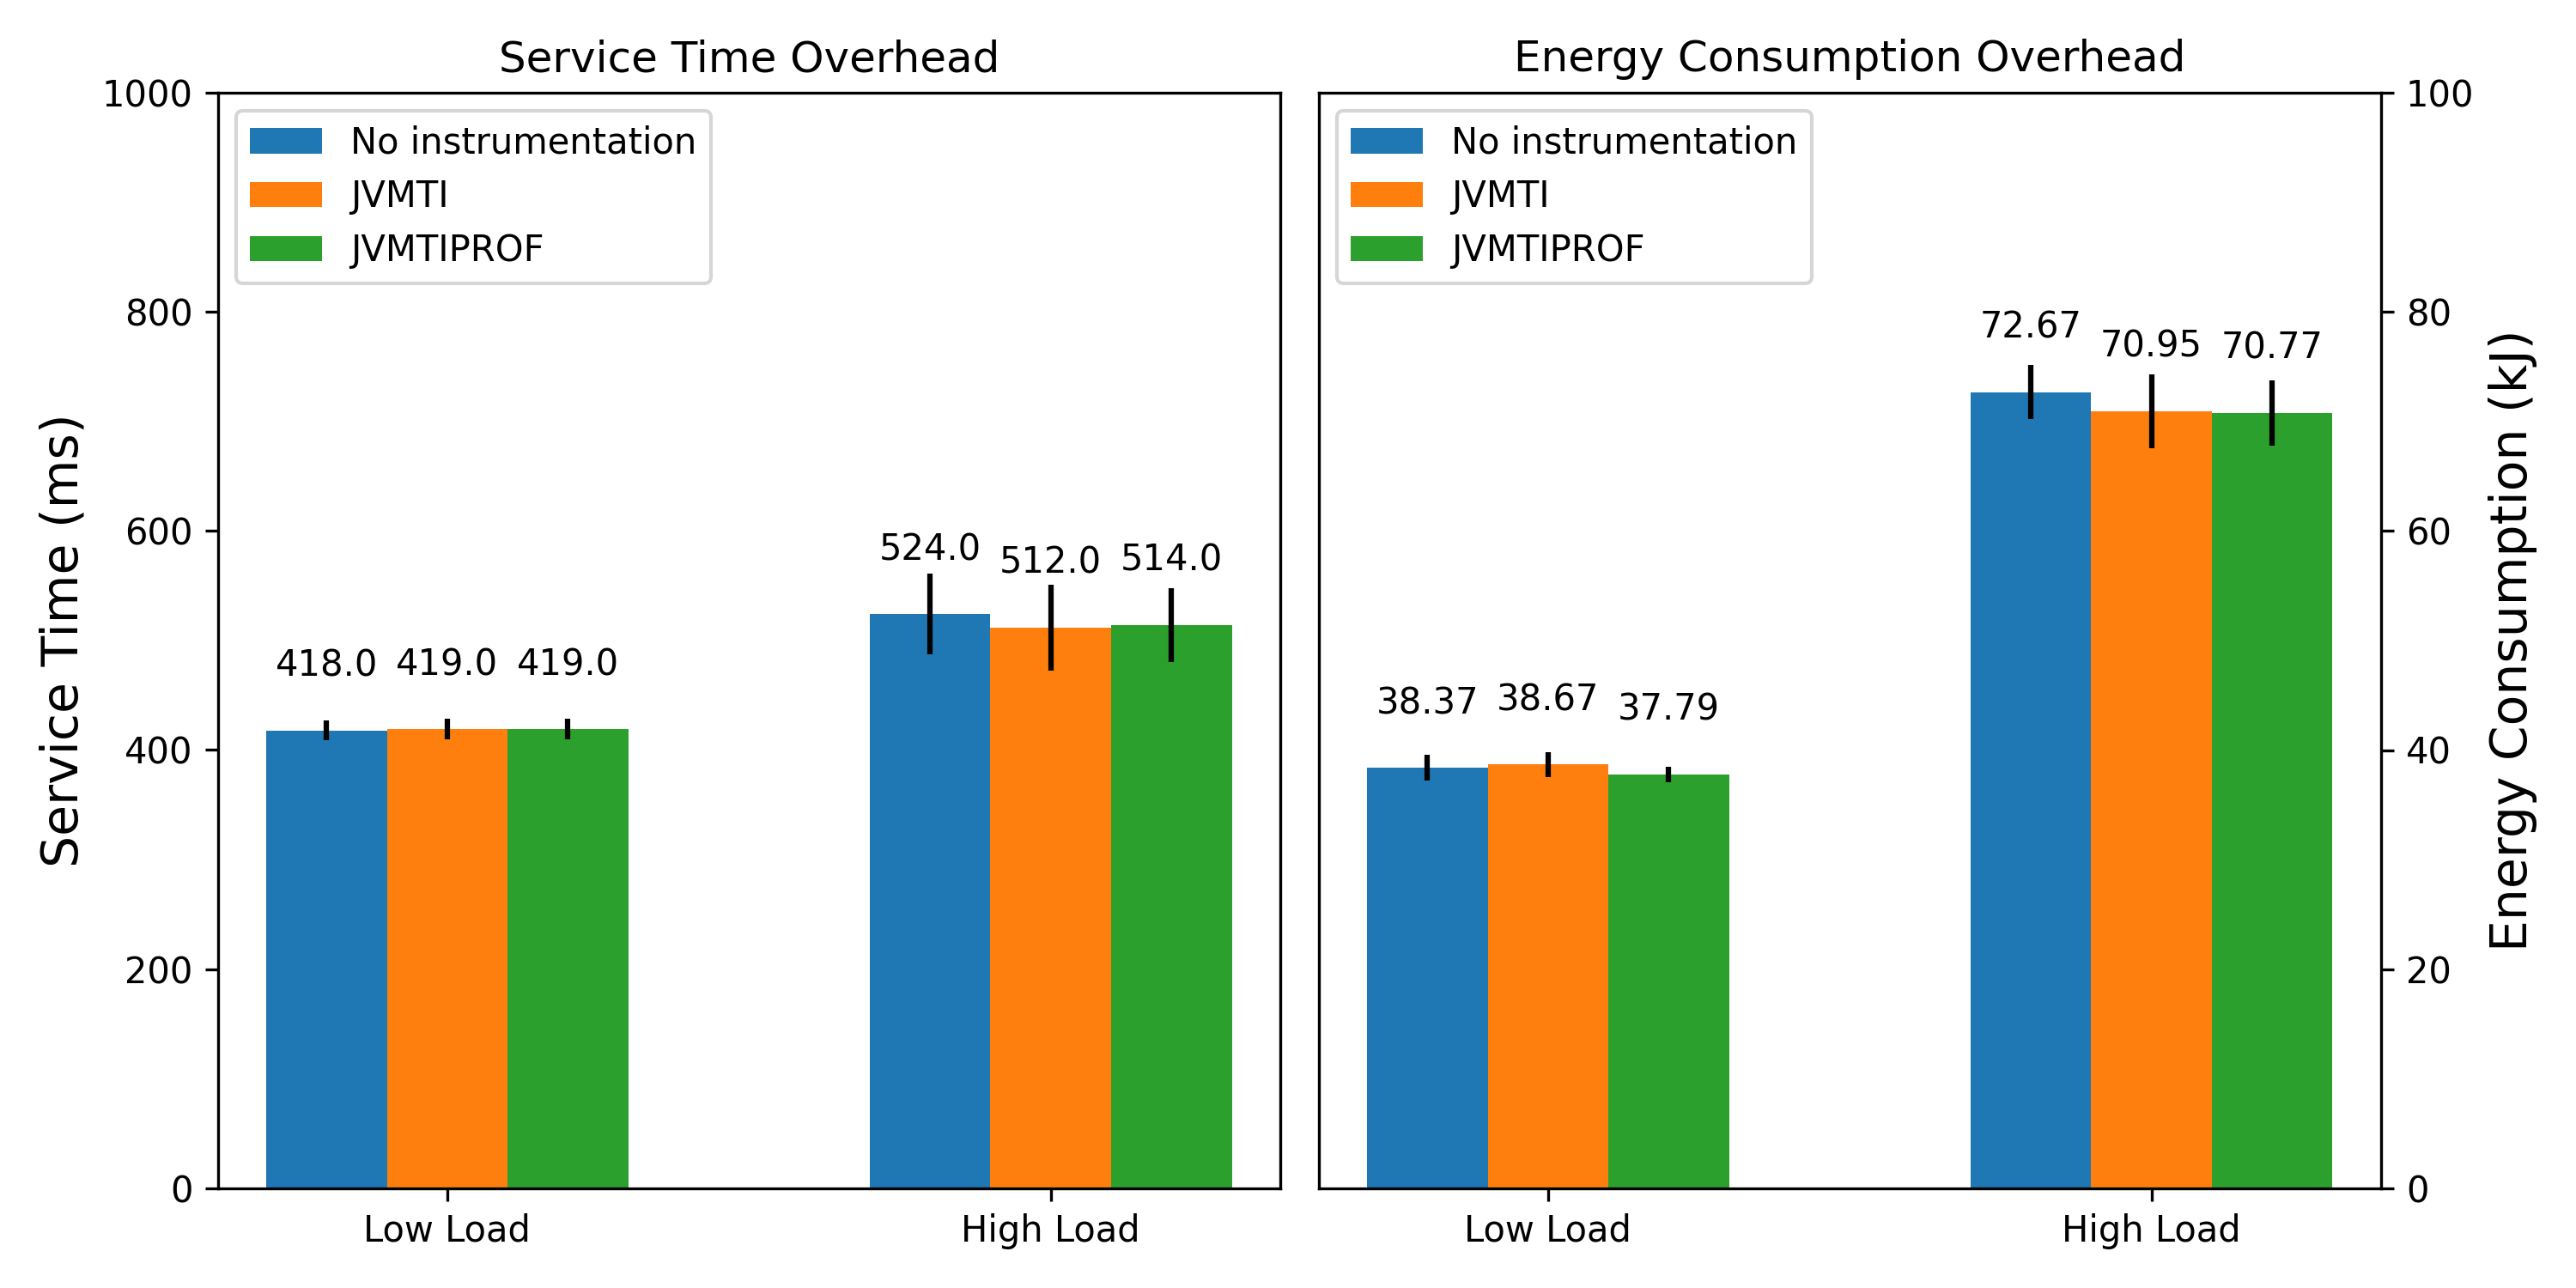
\includegraphics[width=1.0\textwidth]{src/figure/overhead.png}
\caption{An experiment comparing the performance of Elasticsearch when their hot functions are kept as-is or hooked with JVMTI and JVMTIPROF. The left plot presents Elasticsearch's service time, and the right plot the energy consumption of the CPU while executing search requests. Results are shown for both a low and high server load.}
\label{fig:overhead}
\end{figure}

These results also show that the context in which the instrumentation is used may cause performance differences. When instrumenting to run Hurryup at a higher load, JVMTIPROF performed worse than JVMTI, but no difference is seen at lower loads or with scheduling logic removed.

\xchapter{Concluding Remarks}{}
\label{cap:conclusion}

This work presented the design and implementation of JVMTIPROF, an extension to JVMTI with higher-level functionalities. We evaluated the framework in an existing system and found minimal penalties compared to pure JVMTI.

We have also shown how JVMTI can be extended by manipulating its function table. In our experience, the technique is overly complex and hard to maintain, suggesting alternative solutions should be favored, such as the creation of a JVMTI environment private to the extended interface.

In the future, cross-platform support and additional functionalities can be explored. The present components have room for improvement as well. Call stack tracing does not expose kernel, and native functions, which can be solved by the hybrid approach of \citeonline{asyncprofiler}. Method interception may be more performant if we generate specialized code for each hook, avoiding the intermediate lookup by an integer identifier. Finally, execution sampling may benefit from a per-thread timer instead of an application-wide one.



%% Parte pos-textual
\backmatter

% Bibliografia
% É aconselhável utilizar o BibTeX a partir de um arquivo, digamos "biblio.bib".
% Para ajuda na criação do arquivo .bib e utilização do BibTeX, recorra ao
% BibTeXpress em www.cin.ufpe.br/~paguso/bibtexpress
\bibliographystyle{abntex2-alf}
\bibliography{src/biblio}

% Apendices
% Comente se naoo houver apendices
%\iffalse
%\appendix

%\xchapter{Exemplo de Apêndice}{} %sem preambulo
%\lipsum
%\fi
% Eh aconselhavel criar cada apendice em um arquivo separado, digamos
% "apendice1.tex", "apendice.tex", ... "apendiceM.tex" e depois
% inclui--los com:
% \include{apendice1}
% \include{apendice2}
% ...
% \include{apendiceM}

%% Fim do documento
\end{document}
%------------------------------------------------------------------------------------------%
